\documentclass{article}
\usepackage{graphicx} % Required for inserting images
\usepackage[margin=1in]{geometry}
\usepackage{amsmath}
\usepackage{amsfonts}
\usepackage{amsthm}
\usepackage{thm-restate}
\usepackage[]{hyperref}
\usepackage{cleveref}
\usepackage{xcolor}
\usepackage{bbm}
\usepackage{dirtytalk}
\usepackage{graphicx}
\usepackage{subcaption}
\usepackage{float}

\declaretheorem[name=Theorem,numberwithin=section]{thm}
\declaretheorem[name=Lemma,numberwithin=section]{lemma}
\declaretheorem[name=Assumption,numberwithin=section]{asmpt}
\declaretheorem[name=Proposition,numberwithin=section]{prop}
\declaretheorem[name=Corollary,numberwithin=section]{corollary}
\declaretheorem[name=Remark,numberwithin=section]{rmk}
\declaretheorem[name=Definition,numberwithin=section]{defn}

\newcommand{\man}{\mathcal{M}}

\definecolor{cyan}{cmyk}{1, 0.4, 0, 0} 
\newcommand{\ndfg}[1]{{\color{cyan}[Florian: #1]}}

\usepackage[numbers]{natbib}
\bibliographystyle{unsrtnat}

\title{Parallel Transport on WFR$(\mathbb{R}^d)$}
\author{Florian Gunsilius, Gonzalo Mena, Tristan Saidi, Larry Wasserman}

\begin{document}

\maketitle

\section{Genomics setup}

We can describe two relevant genomics scenarios. In either case, for either the treated ($X$) or control $(Y)$ groups, we will have that $X$ and $Y$ can be represented as arrays $X^t$, $t=1,\ldots T_x$, $Y^t$, $t=1,\ldots T_y$. In turn, each of $X^t$, $Y^t$ are positive matrices of dimensions $(n_{t,x},G)$ and $(n_{t,y},G)$ respectively. $n_{t,x}$ and $n_{t,y}$ are the number of profiled cells at time $t$ and $G$ is the number of "genes". The variable $t$ represents temporal indexing although the relationship with biological time may not be straightforward, and may differ in treatment and control groups. Each entry $X^t_{i,j} $ is the number of times gene $j$ (or a mRNA proxy for it more precisely) was read in cell $i$ in the treated (or control) groups. Although raw counts are counts they can be turned into real/positive by usual normalization and take the entire real range by suitable further logarithmic transformations.

\subsection{Development setup}
Here we describe the setup of \citep{shen2025pluripotent}. There is a single control group where cells are measured at $t=1,\ldots 9$ days. There are 9 treated groups, each corresponding to a different genomic perturbation. These perturbations are applied at time $t=2$ from a distribution that is identical to control prior to this period. \ndfg{QUestion for Gonzalo: so between t=1 and t=2 cells evolve differently already, right? They are perfectly equal at t=1 and then at t=2 is the ``baseline'' where treatment is assigned? This means that it would fit our setup perfectly: since treatment is not assigned at t=1, the two cells will in general be slightly different when treatment is assigned at the ``baseline'' t=2, right? But they should still be very similar in terms of the WFR distance such that the "causal model" I persented at the JSM would fit perfectly. My question is if my assessment is correct here. }


\begin{figure}
\begin{center}
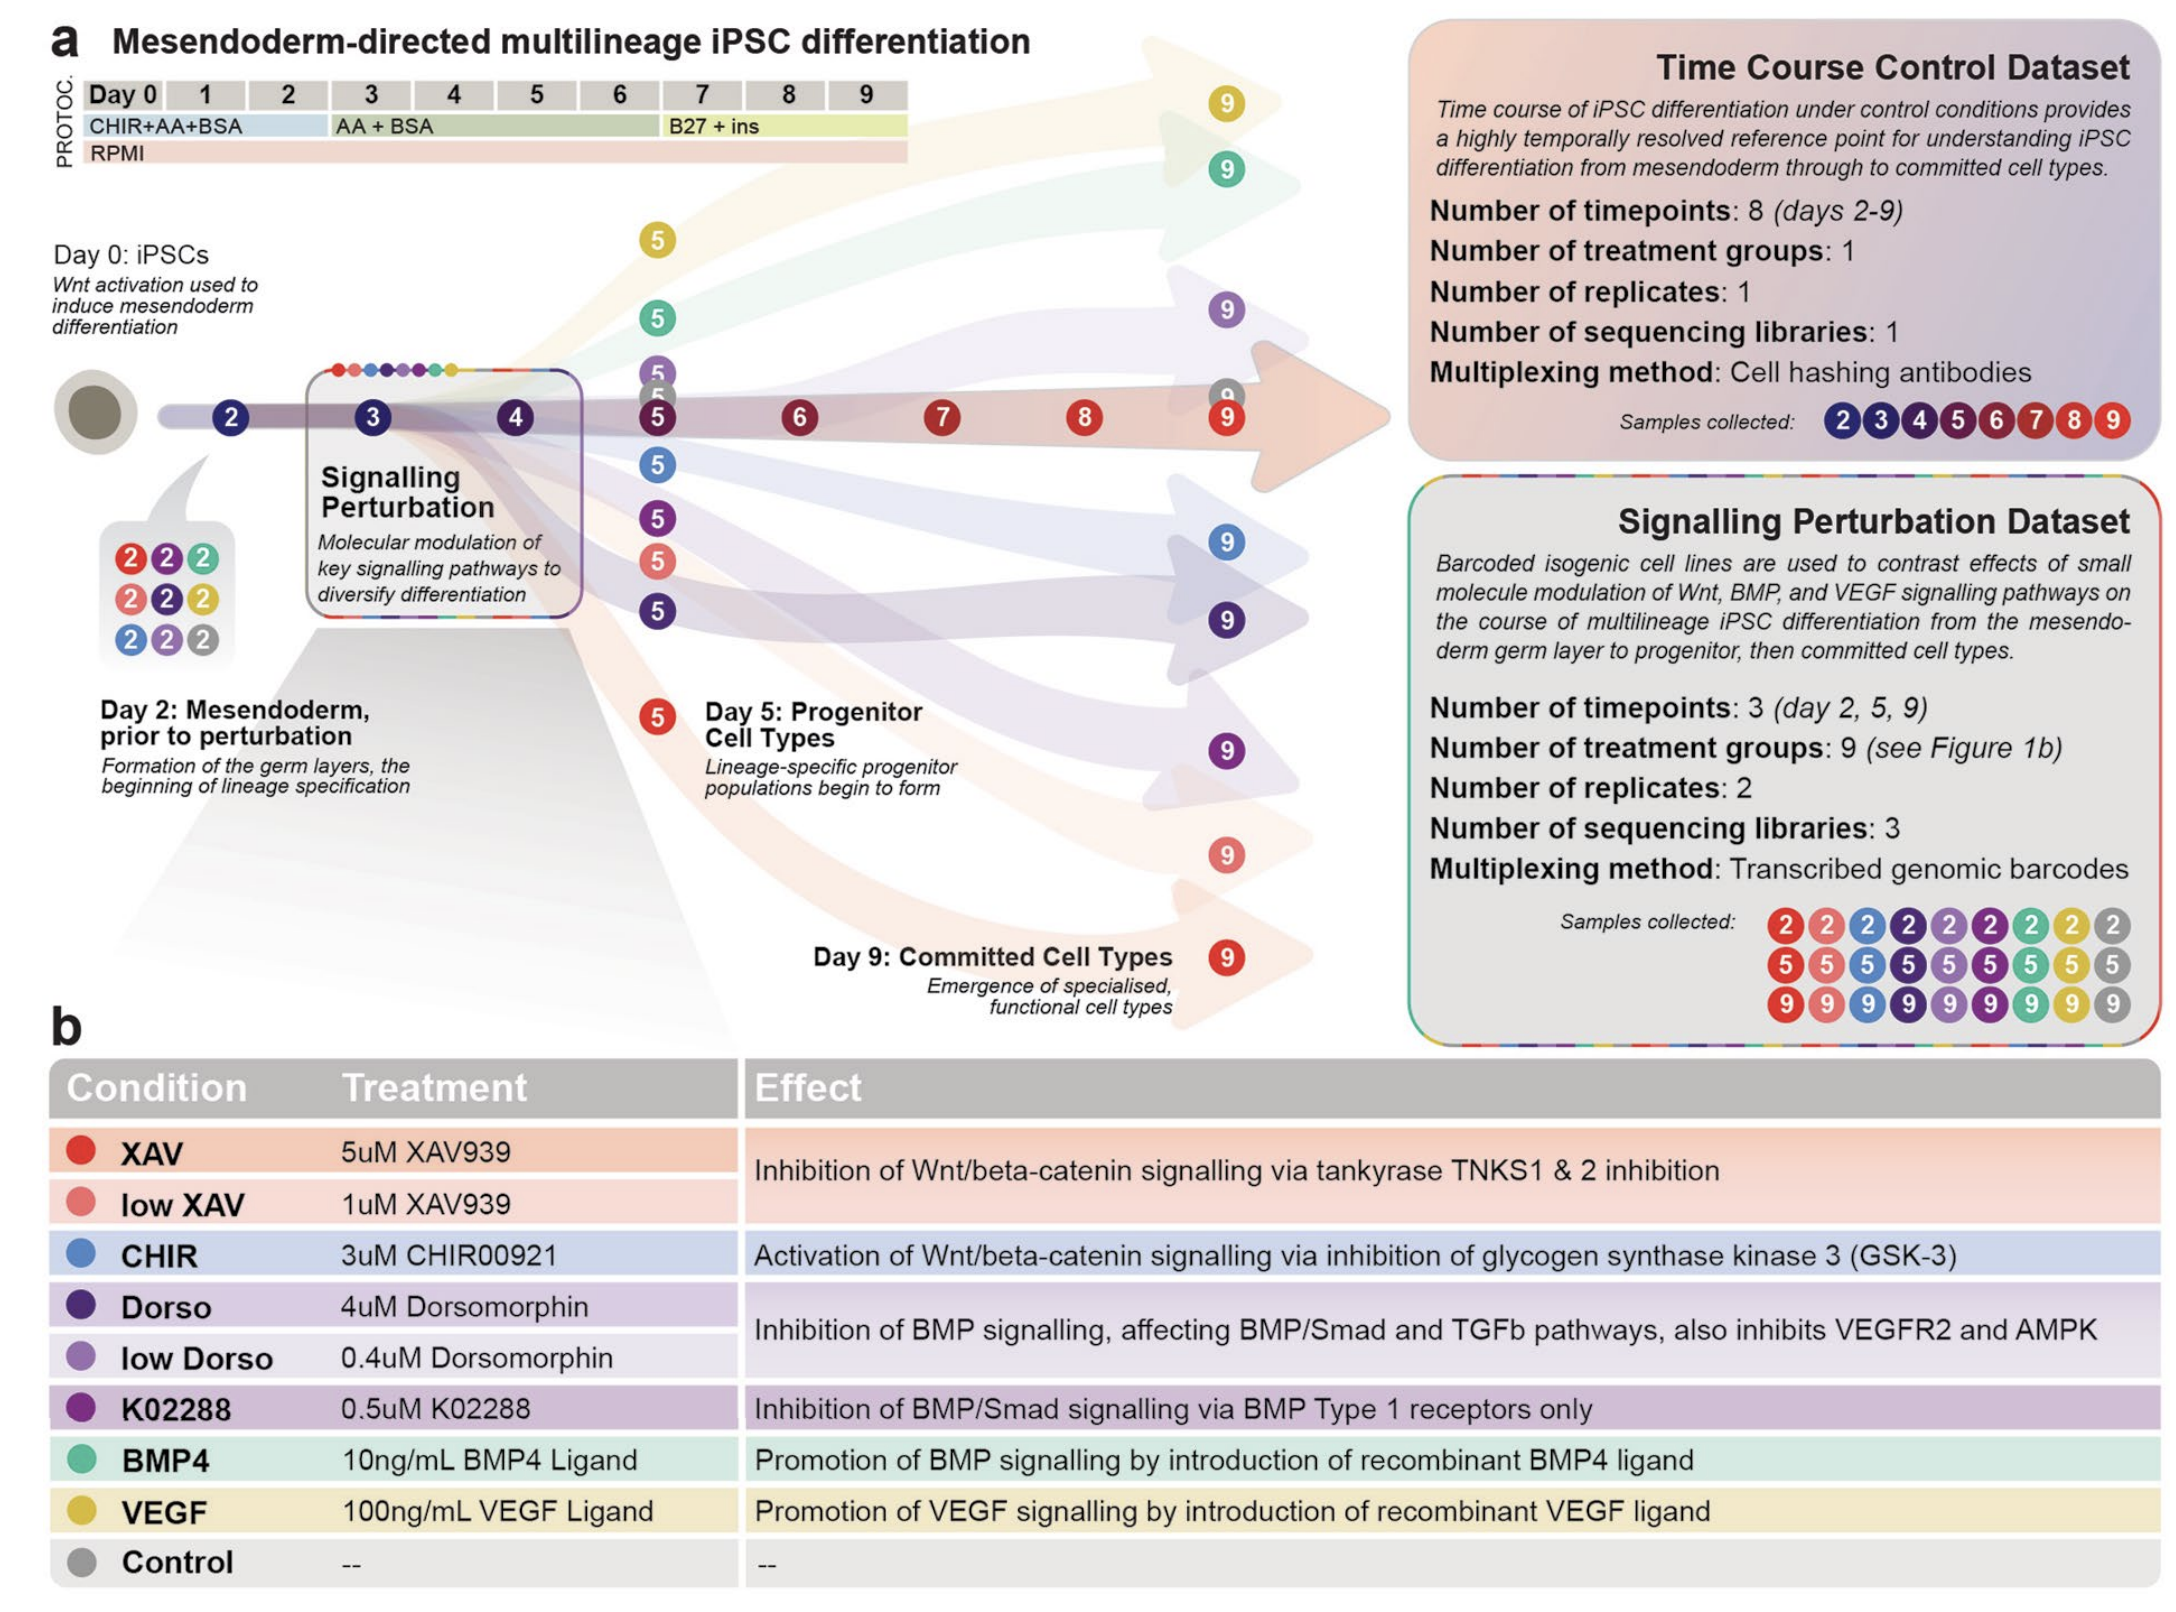
\includegraphics[scale=.4]{Figures/developmentShi.png}
\end{center}
\vspace{-1cm}
\caption{Setup of \citep{shen2025pluripotent}}
\label{fig::Rectangle_Plot}
\end{figure}
\subsection{Alzheimer's disease setup}
This is more challenging. In this case we aim to compare two groups defining a treatment. For example, this may correspond to the presence of a genomic variant such as APOE3. For each treated and control group, we have matrices of gene expression encompassing $ T_x$ and $ T_y$ donors, respectively. Each of these matrices shows gene expression profiling of the brain at autopsy. 

Compared to the Development setup, this is more challenging for several reasons. First, donors are not aligned with progression time; this variable must be inferred. Second, if times were known, there are many other confounding variables (e.g. demographics) that need to be accounted for. Third, there may be heterogeneity in how the sampling is done for each donor (e.g. different slices of the brain). Fourth, here the treatment is assigned at birth. Fifth, the time-scales and sampling rates involved (years) may make it harder to detect causal changes with precise timing.
{\bibliography{main.bib}}

\end{document}
